% !TeX program = pdflatex
% IEEE JBHI submission -- basato su IEEE-TJ-color-latex-template (ieeecolor)
\documentclass[journal,twoside,web]{ieeecolor}
\usepackage{generic}
% Sostituire "generic" con il file di stile della rivista (es. \usepackage{jbhi})
% quando disponibile; nel frattempo si imposta il nome della testata a mano:
\def\journalname{IEEE JOURNAL OF BIOMEDICAL AND HEALTH INFORMATICS}

\usepackage{cite}
\usepackage{amsmath,amssymb,amsfonts}
% amsthm omesso: ieeecolor definisce gia' \proof
\usepackage{mathtools}
\usepackage{graphicx}
\usepackage{textcomp}
% Le figure sono PDF vettoriali esterni in figures/ (sorgenti TikZ inclusi).
\usepackage{xurl}
\usepackage{hyperref}
\hypersetup{hidelinks}

% The legacy color template otherwise places its first-page banner in a
% column-width output box under current LaTeX, producing a large overfull box.
\makeatletter
\def\ps@titlepagestyle{%
  \def\@oddhead{}\def\@evenhead{}%
  \def\@oddfoot{}\def\@evenfoot{}}
\makeatother

\setlength{\textfloatsep}{6pt plus 2pt minus 2pt}
\setlength{\floatsep}{4pt plus 2pt minus 2pt}
\setlength{\intextsep}{6pt plus 2pt minus 2pt}
\setlength{\abovecaptionskip}{4pt plus 1pt minus 1pt}
\setlength{\belowcaptionskip}{2pt plus 1pt minus 1pt}

\newtheorem{theorem}{Theorem}
\newtheorem{definition}[theorem]{Definition}
\newtheorem{property}[theorem]{Property}

\newcommand{\set}[1]{\{#1\}}
\newcommand{\powerset}{\mathcal{P}}
\newcommand{\tuple}[1]{\langle #1 \rangle}

% Layout finale: la tabella del matched campaign (RQ2/RQ4) e' riportata
% nel corpo visibile del testo, essendo il risultato quantitativo
% principale del paper. La tabella e la figura di scaling restano
% disattivate nel layout principale: i valori chiave sono riportati in
% prosa e il dettaglio completo delle otto configurazioni resta nel
% pacchetto di riproducibilita'
% (si_scaling_sweep_2026/scripts/make_figures.py).
% La figura di routing resta disattivata per evitare di duplicare la
% tabella MAUDE e il riepilogo testuale dello stesso trade-off.
\newif\ifrqtwotable  \rqtwotabletrue
\newif\ifrqtwoplot   \rqtwoplotfalse
\newif\ifscalingtable \scalingtablefalse
\newif\ifscalingplot  \scalingplotfalse
\newif\ifroutingplot  \routingplotfalse

\markboth{\hskip25pc IEEE JOURNAL OF BIOMEDICAL AND HEALTH INFORMATICS}
{Author \MakeLowercase{\textit{et al.}}: BioDevOps: An Assurance Architecture for Bounded Agentic Evidence Assembly}

\begin{document}

\title{BioDevOps: An Assurance Architecture for Bounded Agentic Evidence Assembly in Medical-Device Governance}

\author{First A. Author, Second B. Author, and Third C. Author
\thanks{Manuscript received XX Month 2026; revised XX Month 2026. This work received no external funding. (\textit{Corresponding author: First A. Author.})}
\thanks{The authors are with the Department, Institution, City, Country
(e-mail: contact@institution.edu).}}

\maketitle


\begin{abstract}
Agentic artificial intelligence can accelerate evidence retrieval and synthesis in medical-device governance, but safeguards must separate automated recommendations from accountable release authorization. We present BioDevOps, an assurance architecture for bounded agentic evidence assembly. A typed \textit{RiskReport} links a bounded agent to an evidence graph; Open Policy Agent enforces evidential and procedural requirements; the Shapes Constraint Language checks reports against curated clinical facts and can trigger one revision; and a modeled external interface represents human release authority. We evaluated it with Alloy and TLA+, conformance and mutation tests, and 2,000 attempted runs across ten open-weight models on synthetic, public post-market, model-scale, and cross-domain benchmarks. No counterexample to the specified autonomy, accountability, or evidence-mediation properties was found within the explored scopes. Of 2,000 attempts, 1,947 produced reports terminating as advisory packages or governed escalations; no terminated trace accepted a schema-invalid, unparsable, or state-illegal action. On 20 held-out public device reports, enforcement changed under-routing from 2/20 to 0/20 while over-routing reached 14/20. Across three models, 16 of 39 consistency-triggered revisions changed severity or recommendation, without necessarily resolving all nonconformities. Under the evaluated conditions, automated evidence assembly remained inspectable and distinct from the modeled authorization interface.
\end{abstract}

\begin{IEEEkeywords}
Agentic artificial intelligence, formal methods, healthcare governance, human oversight,
medical device software, policy as code, trustworthy artificial intelligence.
\end{IEEEkeywords}

\section{Introduction}
\label{sec:introduction}
\IEEEPARstart{A}{gentic} artificial intelligence can inspect records, retrieve artifacts, and synthesize validation recommendations. In medical-device validation, this makes the boundary between evidence production and release authority a first-order governance problem: trustworthy-healthcare frameworks require traceability, accountability, and human oversight~\cite{future_ai,nist_ai_rmf,eu_ai_act}, while device regulation requires validation, risk management, and controlled change~\cite{fda_aiml_2021,fda_pccp_2025,eu_mdr}. Realizing autonomous, trustworthy, and human-centric agentic systems in healthcare therefore requires an architecture, not only a capable model: one that makes agent autonomy, safety, and accountable human oversight structurally verifiable rather than aspirational. Such governance mechanisms can support future evaluation of agentic AI in clinical and home-care environments, where automated evidence work must remain auditable under regulatory, ethical, and privacy constraints.

Authority becomes ambiguous when advice is treated as a decision, cited material does not support its claim, or review lacks a record of the human decision. An assurance architecture must therefore separate advice from approval, preserve claim-to-evidence paths, and expose unresolved conditions before release.

The agent produces an advisory \textit{RiskReport}; Open Policy Agent (OPA) checks evidential and procedural conditions and routes it for human review, while authorization remains with a modeled--not integrated--external service. An evidence graph links clinical events, artifacts, tests, obligations, and review actions. The Shapes Constraint Language (SHACL) provides post-hoc consistency analysis and a controlled one-revision path; Alloy/Temporal Logic of Actions (TLA+) models and conformance/mutation tests examine structural, temporal, and operational properties.

This paper makes three contributions:
\begin{itemize}
\item an evidence-to-authority architecture with formally checked invariants that assign recommendation and authorization to separate objects, actors, and controls;
\item a bounded evidence-assembly agent and typed contract combining traceable trajectories, deterministic transitions, OPA enforcement, and SHACL analysis; and
\item a multi-method evaluation spanning extended formal scopes, 2,000 attempted runs across ten models, field provenance, mutation-sensitive tests, public Manufacturer and User Facility Device Experience (MAUDE) reports, and cross-domain transfer, providing inspectable evidence for evaluating agentic-AI governance claims.
\end{itemize}

\paragraph{Study scope.} We evaluate reviewer decision rights, traceability, bounded agent behavior, and accountable routing against reproducible developer-authored governance references. Human reliance, clinical effectiveness, and authenticated production integration require separate evaluation.

A preliminary version of this work has been reported~\cite{mirto_biodevops_phdforum}.

\section{Related Work}

Trustworthy-AI frameworks call for traceability, accountability, oversight, fairness, usability, and robustness~\cite{future_ai,future_ai_review,nist_ai_rmf,eu_ai_act}. Device guidance, the EU MDR, and ISO standards add validation, risk-management, change-control, and AI-management duties~\cite{fda_aiml_2021,fda_pccp_2025,eu_mdr,iso13485,fda_gmlp,iso14971,iso42001,nist_genai_profile}; RegOps brings such controls into deployment pipelines~\cite{toivakka_regops}. We provide an executable counterpart: developer-authored OPA and SHACL controls motivated by ISO~14971 and GMLP. Preliminary BioDevOps work~\cite{mirto_biodevops_phdforum} separated evidence production from authorization; this article makes that boundary agent-specific, executable, formally checked, and empirically evaluated.

Agentic systems combine planning, retrieval, and tools~\cite{lewis_rag,yao_react}; healthcare benchmarks probe them in simulated clinical and EHR tasks~\cite{agentic_taxonomy_2026,agentclinic,medagentbench}, while structural critiques emphasize accountable oversight~\cite{agentic_limits_2026}. Complementary JBHI work operationalizes trustworthy-AI guidance, diagnostic retrieval, and public-EHR benchmarking~\cite{future_ai_review,garmle_g,public_ehr_benchmark}; we govern the combination of retrieval, evidence assembly, generation, and intermediate decisions before release. Automation-bias and clinical studies show that workload, expertise, presentation, and incorrect advice affect reliance~\cite{goddard_automation_bias,gaube_do_as_ai_say,tschandl_collaboration}. Reporting standards and organizational governance frameworks address adoption and oversight~\cite{decide_ai,economou_zavlanos_jamia,wang_governance_scoping}; we complement them with an executable boundary where agent-produced evidence meets human authority.

Our neuro-symbolic design evaluates a fixed report contract against FHIR-shaped data, SNOMED CT mappings, and closed-world SHACL constraints~\cite{liu_snomed_kg,fhir,snomed,shacl,owl2}; bounded models and runtime tests examine authority and evidence properties~\cite{leucker_runtime}. Policy-as-code gates deployment artifacts~\cite{opa_cicd,github_environments,toivakka_regops}, whereas agent guardrails constrain dialogue and tools~\cite{nemo_guardrails,agentspec}. Neither checks generated evidential claims against curated clinical facts before human authorization in the setting targeted here. We compare direct generation, RAG, bounded-agent, and OPA-governed arms over identical scenarios (Section~\ref{sec:agent-evaluation}).

The preliminary two-page report~\cite{mirto_biodevops_phdforum} presented the state formula, admissibility condition, and qualitative insulin-pump scenario as a narrative specification, leaving tool encoding and evaluation as future work. This article adds Alloy and TLA+/TLC models, executable OPA/SHACL controls, an agent-specific bounded runtime, mutation-sensitive tests, 2,000 attempted runs across ten models, public post-market evaluation, and cross-domain and paraphrase transfer.

\section{Formal Architecture Model}
\label{sec:architecture}

Telemetry, drift alerts, performance monitors, and post-market reports enter release decision-making only as reviewed, traceable evidence. The prototype implements report generation and routing; its external authorization interface is modeled--not integrated.

Building on BioDevOps~\cite{mirto_biodevops_phdforum}, we represent governance as $P=(C,\Delta,R,V,E,G)$: changed components, change class, risk, validation path, evidence, and governance. Traceable $Artifact$, $Stage$, $RiskSignal$, and $Gate$ structures connect claims to their producing change and stage. \textit{Human Accountability} requires each \textit{ApprovalRecord} to trace to an authorized human; the \textit{AI Autonomy Constraint} permits evidence gathering and recommendation but excludes execution and deployment; and \textit{Evidence-Mediated Governance} requires evidence and authorized approval for gate transitions. Section~\ref{sec:formal-verification} verifies these properties at extended bounds.

Pipeline stages emit validation or failure evidence; gates evaluate evidence, signatures, and policy. Riskier ML changes add drift, calibration, subgroup, simulation, or software-/hardware-in-the-loop evidence~\cite{iec62304}. Agents request evidence-producing stages, whereas approval records originate at the external human gate.

\section{Knowledge-Guided Agent}
\label{sec:agentic-ai}

\begin{figure}[t]
\centering
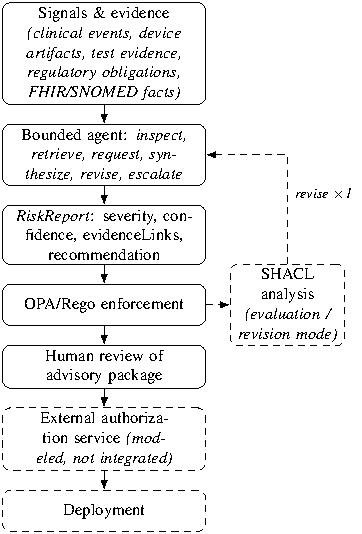
\includegraphics[width=0.85\columnwidth]{figures/fig1_architecture.pdf}
\caption{Evidence-to-authority flow. OPA governs the advisory path to human review; evaluation-layer SHACL analysis can condition one bounded revision. Only the external authorization service can mediate deployment.}
\label{fig:architecture}
\end{figure}

An evidence directed acyclic graph (DAG) connects clinical events, device artifacts, tests, obligations, and FHIR/SNOMED facts to the \textit{RiskReport} and human review (Figure~\ref{fig:architecture}). The agent inspects signals, retrieves or requests artifacts, drafts a report, and revises once or escalates. Its actions are $\{\textit{inspect},\textit{retrieve},\textit{request},\textit{synthesize},\textit{revise},\textit{escalate}\}$; validation, approval, and deployment are excluded. Actions record sources and outcomes, and allow-listed tools return evidence or failure records.

The model proposes actions, queries, or evidence requests; the runtime validates transitions, executes allow-listed tools, limits trajectories to six steps and one revision, applies OPA/SHACL, and escalates unresolved paths. JSON Lines (JSONL) traces record proposed and accepted actions, state hashes, retrieved identifiers, gaps, policy actions, configuration metadata, and termination. Thus, model-guided assembly remains under deterministic runtime control.

Report claims use typed evidence paths. The DAG records each artifact's role, supported claim, provenance, contradictions, and missing dependencies, distinguishing authentic but irrelevant evidence from direct support. Citation validity therefore differs from evidential sufficiency and release authority.

The contract is $Input=\powerset(Artifact)\times\powerset(RiskSignal)$ and $Output=RiskReport=\tuple{severity,confidence,evidenceLinks,recommendation}$. Recommendations range from \textit{NoAction} to \textit{EscalateImmediate}; none authorizes deployment. Claims link to signed evidence marked sufficient, weak, or absent, and report signatures record provenance rather than approval.

Determinism concerns enforcement, not generation: given a \textit{RiskReport}, transition validation, trajectory bounds, OPA/SHACL application, and the external gate are deterministic (Section~\ref{sec:formal-verification}). Report content remains subject to decoding, serving, and model drift; the measured 72-hour same-digest variation is quantified under Threats to Validity. The in-loop path (Section~\ref{sec:inloop-revision}) re-invokes the model, but the runtime still bounds the revision.

Two symbolic analyses operate at different stages. OPA/Rego enforces citation, escalation, field-action, and routing rules over the generated report. SHACL compares stored reports with curated FHIR-shaped facts and SNOMED CT mappings; the OWL 2 Web Ontology Language RL profile (OWL-RL) selects one-sided severity constraints. For example, confirmed ventricular fibrillation (SNOMED CT 71908006) makes \textit{NoAction} or \textit{Monitor} nonconformant.

OPA resolves identifiers and procedural conditions; SHACL compares typed assertions with fixed facts. Together they expose citation failures, missing evidence, severity under-calls, and graph contradictions. Assertion status---confirmed, suspected, negated, or mention-only---drives the continuous glucose monitoring (CGM) transfer experiment (Section~\ref{sec:cgm-generalization}).

Ordinal checks are one-sided: severity-floor, severity-4/death, and CGM confirmed-event rules flag under-triage, prioritizing missed escalation over extra review. A separate rule flags unsupported field-safety action to address unwarranted recall. Section~\ref{sec:model-scale-sensitivity} examines this asymmetry's coverage gaps empirically.

The self-reported \textit{confidence} field is routing metadata, not severity or a policy verdict. OPA combines it with citation, support, completeness, and escalation checks; authorization never depends on it.

OPA normalizes drafts by adding review, escalation, or missing-evidence actions; SHACL annotates the curated graph. The advisory package separates recommendation, sources, gaps, and policy actions, while release decisions remain external.

When measuring OPA-or-SHACL trigger yield, Section~\ref{sec:synthetic-40} disables universal review so that this routing invariant is not counted as check performance.

\section{Bounded Formal Verification and Operational Conformance}
\label{sec:formal-verification}

The three properties retain passing results at larger bounds. Deployment requires complete, traceable, human-approved evidence:
\begin{IEEEeqnarray}{rCl}
deploy(P) &\Rightarrow& approved(G) \land complete(V,E) \IEEEnonumber \\
&\land& traceable(E,C,\Delta). \IEEEyesnumber
\label{eq:deploy-admissible}
\end{IEEEeqnarray}
The bounded temporal model checks a narrower risk-mediation condition over pending risks, $PendingRisk(P)\subseteq RiskSignal$:
\begin{equation}
\begin{split}
\Box\big(&(\exists r\in PendingRisk(P): \neg reviewed(r,E,G))\\
&\Rightarrow \neg authorized(P)\big),
\end{split}
\label{eq:evidence-mediation-safety}
\end{equation}
Under fair scheduling, pending risks eventually reach review, and new unreviewed risk revokes authorization. Alloy checks structure, TLA+/TLC temporal behavior, and Python enumeration provides a bounded cross-check. No encoded scope permits agent deployment, unauthorized approval, or authorization with unreviewed risk; operational tests exercise the corresponding report and routing controls.

The bounded checks verify $approved(G)$, $reviewed(r,E,G)$, and $authorized(P)$ against the variables the models track: $authorized(P)$ is a global Boolean, set by a \textit{GrantAuthorization} transition exactly when every pending risk signal is reviewed; $reviewed(r,E,G)$ is a per-signal Boolean toggled by a \textit{ReviewRisk} transition, treating review as an atomic action rather than separately modeling $E$ and $G$; and the Alloy autonomy model checks $approved(G)$ as gate-set membership, granting execution capability only when a human actor holds an approved gate. Eq.~\eqref{eq:deploy-admissible}'s $complete(V,E)$ and $traceable(E,C,\Delta)$ conjuncts state the report contract's structural guarantees---typed evidence links, provenance fields, and schema validation (Section~\ref{sec:agentic-ai})---enforced by the runtime rather than checked as separate temporal-logic predicates in this section.

At extended scope, autonomy held across 514--12,292 BFS states and Alloy remained UNSAT at 2$\times$ atom scope (6.3s); evidence mediation held across 13--275 states with exact TLC/Python agreement; and accountability held across 25--625 configurations with Alloy UNSAT at 3.3$\times$/2.5$\times$ scope. Violating controls produced counterexamples. Base scopes were \texttt{6 Time, 6 SystemState, 4 Actor, 2 Stage, 2 Component, 1 Gate2} and \texttt{6 Artifact, 4 Actor}; witnesses \texttt{sanityChainIsNontrivial} and \texttt{sanityApprovalRecordsCanExist} guard against vacuity. Construct Validity states the full-scope semantic caveat.

The formal-to-operational mapping pairs each property with an executable check and mutation oracle. AI autonomy is enforced by schema rejection of authority fields, including injected \texttt{release\_authorized}; human accountability by mandatory review routing, whose disabled default exposes an unreviewed report; and evidence mediation by missing-evidence denial plus SHACL checks, for which a weakened constraint fails. The trusted boundary comprises the schema, policy engine, curated facts, and external authorization service, assuming equivalent enforcement at external APIs, no bypass path, truthful inputs, and authenticated approvers. Factual completeness, human judgment, usability, identity, and production integration remain outside the prototype.

Negative controls expose vacuous invariants, disconnected states, reflexive steps, and short cycles; tests also detect mutations removing authority rejection, universal review, or technical-evidence constraints. The formal and executable checks therefore connect the advisory package to human review while authorization remains external.

\section{Evaluation}
\label{sec:agent-evaluation}

We ask whether the architecture preserves the advice--authorization boundary (\textbf{RQ1}), what behavior appears in bounded-agent traces (\textbf{RQ2}), which defects OPA and SHACL detect separately and jointly (\textbf{RQ3}), and how enforcement changes routing, agreement, and review workload (\textbf{RQ4}). Formal analysis addresses RQ1 at the architectural level; the following experiments address all four questions operationally.

\paragraph{Claims and non-claims.} Absolute agreement rates in this section characterize the small open-weight generators under a strict conjunctive metric, not the architecture: the central claims concern boundary preservation and routing under enforcement, and none of the results below establishes clinical correctness or human reliance (Threats to Validity).

\subsection{Setup}
\label{sec:eval-setup}

The primary benchmark contains 40 synthetic, non-patient arrhythmia bundles generated from a fixed template and governance rubric. It balances severity levels 1--4 and covers five recommendations, four evidence-completeness classes, four SNOMED CT concepts, and seven symbolic-check probes. A frozen 20/20 development/held-out split supports one unmodified held-out run. Eight paraphrases of each of five base scenarios form a separate 40-row stability check (Section~\ref{sec:paraphrase-robustness}).

A second frozen cohort contains 40 public MAUDE post-market reports, again split 20/20~\cite{fda_maude}. Annotation retained source digests, explicit facts, and assertion status (\textit{confirmed}, \textit{suspected}, \textit{negated}, or \textit{mention-only}). Two team members independently labeled source narratives without access to generated reports or symbolic findings, followed by third-author adjudication. Development/held-out pre-adjudication Cohen's $\kappa$ was 0.72/1.00 for status, 0.90/0.74 for routing (quadratic-weighted), and 0.78/0.88 for evidence sufficiency. The released protocol, disagreements, and adjudication record make this internal governance reference reproducible.

No human participants or identifiable private information were involved (synthetic scenarios and public FDA MAUDE reports only); Institutional Review Board (IRB) approval and informed consent were therefore not required.

The \textit{matched-strict} protocol fixes scenarios, retrieval, prompts, policy, curated facts, and generation settings across arms, varying only the model. Severity is ordinal (1--4); 95\% Wilson CIs use development ($n=20$), held-out ($n=20$), or pooled ($n=40$) scenarios, and recommendation accuracy is agreement with the governance reference. MAUDE, paraphrase, and cross-domain analyses retain the same fixed-scenario discipline with analysis-specific model rosters.

\subsection{Boundary Enforcement (RQ1--RQ2)}
\label{sec:rq1-rq2-boundary}

\subsubsection{Matched Bounded-Agent Campaign}

The bounded planner's action-contract enforcement---revalidating every model-proposed action against the legal transition set (Section~\ref{sec:agentic-ai})---is exercised end to end by the matched campaign, backed by a dedicated regression test and the full 86-test suite.

The model set contrasts Qwen3.5 and Gemma 3 across different tool-use priors. The 1B--27B range targets local open-weight deployment, relevant where governance restricts external processing of device artifacts. Across 2,000 runs, bounded-agent generation latency had a median of 14.3\,s (range 7.4--72.8\,s); policy latency was not instrumented separately. Pinned digests support traceability but did not eliminate serving or sampling variability.

The campaign covers ten models from three series (qwen2.5:7b; qwen3.5, 0.8B--27B; gemma3, 1B--27B) on both splits, comparing direct generation, RAG, bounded-agent output, and OPA-governed output under identical settings. Of 2,000 attempted agent runs, 1,947 yielded reports: 1,189 reached \texttt{advisory\_complete}, 443 agent-proposed escalation, and 315 runtime-forced escalation after a refused second revision. The other 53 failed inside the report tool, all for qwen3.5:2b (70/100 development and 77/100 held-out completions) because pre-report text preceded valid JSON actions. Completion outcomes include all attempts; agreement rates condition on successful generation. Counting failures as non-agreement changes qwen3.5:2b development agreement from 10/70 (14.3\%) to 10/100 (10.0\%) for raw and agent+OPA; held-out agreement remains 0\%. No terminated trace accepted a schema-invalid, unparsable, or state-illegal action.

Governance-exact-agreement jointly matches routing, evidence insufficiency, citation, and contradiction fields, and is therefore stricter than the single-field recommendation agreement reported in Sections~\ref{sec:synthetic-40} and~\ref{sec:cgm-generalization}.\ifrqtwotable{} Table~\ref{tab:rq2-governance} gives exact counts.\fi{} On development data, raw agent output exceeded the strongest non-agentic baseline for seven of nine fully completed models; OPA lowered agreement for five, left three unchanged, and raised qwen3.5:27b. On held-out data, agreement was nonzero for one raw agent versus six OPA-governed models because selected under-routes became reference-consistent escalations. Scenario-cluster-adjusted intervals remain wide, so comparisons are descriptive; qwen3.5:9b's 13$\to$8 change reflects severity-4 and evidence-completeness rules. qwen3.5:2b rates use 70/77 completed reports. Field decomposition and all intervals are in the reproducibility package.

\ifrqtwotable
\begin{table*}[t]
\centering
\caption{RQ2/RQ4 matched campaign: completion and governance-exact-agreement (agreement/completed outputs)}
\label{tab:rq2-governance}
\scriptsize
\setlength{\tabcolsep}{2.5pt}
\begin{tabular}{lcp{0.09\textwidth}p{0.09\textwidth}p{0.09\textwidth}p{0.09\textwidth}p{0.09\textwidth}p{0.09\textwidth}}
\hline
& & \multicolumn{3}{c}{\textbf{Development}} & \multicolumn{3}{c}{\textbf{Held-out}} \\
\textbf{Model} & \textbf{Complete D/H} & \textbf{Best base} & \textbf{Raw} & \textbf{+OPA} & \textbf{Best base} & \textbf{Raw} & \textbf{+OPA} \\
\hline
qwen2.5:7b   & 100/100 & 15/100 & 25/100 & 25/100 & 0/100 & 0/100 & 10/100 \\
qwen3.5:0.8b & 100/100 & 15/100 & 20/100 & 20/100 & 0/100 & 0/100 & 0/100 \\
gemma3:1b    & 100/100 & 15/100 & 14/100 & 14/100 & 0/100 & 0/100 & 0/100 \\
qwen3.5:2b$^\dagger$ & 70/77 & 10/100 & 10/70 & 10/70 & 0/100 & 0/77 & 0/77 \\
gemma3:4b    & 100/100 & 15/100 & 10/100 & 5/100 & 0/100 & 0/100 & 10/100 \\
qwen3.5:4b   & 100/100 & 15/100 & 25/100 & 20/100 & 0/100 & 0/100 & 5/100 \\
qwen3.5:9b   & 100/100 & 15/100 & 28/100 & 14/100 & 0/100 & 13/100 & 8/100 \\
gemma3:12b   & 100/100 & 15/100 & 30/100 & 25/100 & 0/100 & 0/100 & 9/100 \\
gemma3:27b   & 100/100 & 15/100 & 30/100 & 20/100 & 0/100 & 0/100 & 5/100 \\
qwen3.5:27b  & 100/100 & 15/100 & 25/100 & 30/100 & 0/100 & 0/100 & 0/100 \\
\hline
\multicolumn{8}{p{0.94\textwidth}}{\scriptsize Best base is the stronger of direct generation and non-agentic RAG. $^\dagger$qwen3.5:2b denominators reflect completed agent reports; its non-agentic baselines completed 100 runs. qwen3.5:2b's completion numbers are reported at their original run status; a later same-digest reproducibility probe found drift for this model (Threats to Validity). Scenario-cluster-adjusted intervals for all cells are provided in the reproducibility package.} \\
\end{tabular}
\end{table*}
\fi
\ifrqtwoplot
\begin{figure}[t]
\centering
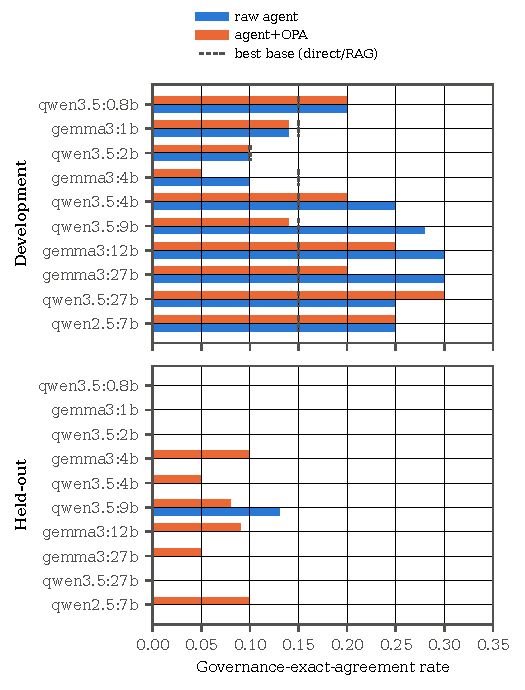
\includegraphics[width=\columnwidth]{figures/fig_matched_campaign.pdf}
\caption{Matched-campaign governance-exact agreement, ten models, development (top) and held-out (bottom). Blue bars: raw bounded agent; orange bars: agent+OPA; the dashed tick marks the best non-agentic baseline (direct generation or RAG) for that model/split. Development best-base is 10--15/100 across models; held-out best-base is 0/100 for all ten models, so the dashed tick sits at the axis origin in every held-out row. $^\dagger$qwen3.5:2b's agent arms use $n=70$/$77$ (development/held-out completions); all other rates use $n=100$, reported at original run status (see Threats to Validity for a later same-digest drift finding on this model). Exact counts, per-field decomposition, and cluster-adjusted intervals are in the reproducibility package.}
\label{fig:rq2-governance}
\end{figure}
\fi

\subsubsection{Frozen Factorial Conformance Suite}
\label{sec:conformance-suite}

An LLM-free suite tested OPA and SHACL against labeled violations. Its 48 prospective rows exposed three defects: substring matching of \texttt{"confirmed"} within \texttt{"unconfirmed"} and two malformed FHIR extensions accepted by SHACL. Exact-phrase and URL/valueCode allowlists repaired all three. The 54-row regression suite adds six technical-evidence cases and tests closure, not unseen-failure generalization. Eligible-row sensitivity rose from 87.5\% to 12/12 for OPA and 16/16 for SHACL (95\% Wilson lower bounds 75.8\% and 80.6\%); class coverage rose from 1/2 to 3/3 and 3/4 to 4/4.

\subsubsection{Structural Boundary Evidence}

Operational results were consistent with the encoded boundary under the tested configurations: no accepted action was invalid or state-illegal in 2,000 runs, structural violations were 0/40 in the frozen benchmark, no paraphrase crossed the authority boundary, and cross-domain transfer produced no unsafe under-escalation. No tested input gave the agent authorization or execution capability.

\subsection{Defect Detection (RQ3)}
\label{sec:rq3-defect-detection}

\subsubsection{Frozen Synthetic 40-Scenario Symbolic-Check Benchmark (OPA/SHACL Detection Decomposition)}
\label{sec:synthetic-40}

With mandatory review disabled, OPA-or-SHACL trigger yield measures the fraction of generated reports flagged by either check. Cross-tabulating OPA (on/off) against SHACL (on/off) over the same 40 scenarios gives a 2$\times$2 decomposition of the two symbolic checks' detections: OPA-only, SHACL-only, overlap, and neither counts attribute each activation on the same generated report, while the structural boundary violation rate evaluates the report contract separately. This decomposes which check catches a defect on the same report; the pipeline is not re-executed with each check disabled, so ablated downstream agent behavior (revision, escalation) is not established.

Under the matched-strict protocol (Section~\ref{sec:eval-setup}), Table~\ref{tab:independent-scenario-level} reports the qwen2.5:3b results, retained as the single-series historical baseline for the two-series scaling sweep (Section~\ref{sec:model-scale-sensitivity}). With routing disabled, union yield is 0.625 (0.350 development; 0.900 held-out).

\begin{table}[t]
\centering
\caption{Frozen 40-scenario benchmark: matched-strict qwen2.5:3b results, pooled (dev.+held-out; union yield split noted in text). OPA-only/SHACL-only/overlap/neither rows form a 2$\times$2 detection decomposition, not an independently re-executed ablation.}
\label{tab:independent-scenario-level}
\scriptsize
\setlength{\tabcolsep}{2.0pt}
\begin{tabular}{p{0.60\columnwidth}p{0.30\columnwidth}}
\hline
\textbf{Metric (scenario-level)} & \textbf{Pooled ($n=40$)} \\
\hline
Severity accuracy & 17/40=0.425 [0.285,0.578] \\
Policy-adjusted agreement with developer reference & 17/40=0.425 [0.285,0.578] \\
Structural boundary violation rate$^\dagger$ & 0/40=0.000 \\
OPA-or-SHACL union yield$^\ddagger$ & 25/40=0.625 [0.470,0.758] \\
OPA-only catches & 16/40 \\
SHACL-only catches & 6/40 \\
OPA/SHACL overlap (structural / genuine)$^{**}$ & 3/40 (2/1) \\
Neither layer catches & 15/40 \\
Raw citation hallucination & 5/40=0.125 [0.054,0.261] \\
\hline
\multicolumn{2}{p{0.94\columnwidth}}{\scriptsize $^\dagger$Structural gate outcome; no interval. $^\ddagger$Review gate disabled; union equals OPA-only + SHACL-only + overlap, with development/held-out yield 0.350/0.900. $^{**}$Overlap is decomposed into shared-field and genuinely independent activation in Section~\ref{sec:guard-independence}. Cluster-adjusted precision is discussed under Threats to Validity.} \\
\end{tabular}
\end{table}

Across qwen2.5:1.5b/3b/7b ($n=40$ per arm), severity accuracy was 0.375/0.425/0.450, governed recommendation agreement was 0.375/0.425/0.425, and union yield was 0.825/0.625/0.900. SHACL-only catches increased from 4 to 6 to 12, showing incremental detection of severity under-calls after OPA had accepted the report's citation and procedural fields. These configurations provide the historical single-series baseline and field-provenance audit trail; the primary cross-series analysis appears in Section~\ref{sec:model-scale-sensitivity}\ifscalingtable{} (Table~\ref{tab:scaling-sweep})\fi\ifscalingplot{} (Figure~\ref{fig:scaling-sweep-multipanel})\fi.

Distinct check capabilities are evaluated separately in the large language model (LLM)-free conformance suite against known defects (Section~\ref{sec:conformance-suite}).

\subsubsection{Symbolic-Check Independence and Field-Sharing Effects}
\label{sec:guard-independence}

We trace each active OPA rule and SHACL shape to its \textit{RiskReport} field, classifying overlap as \textit{structurally redundant} when both layers read the same field and condition, or \textit{genuinely independent} otherwise.

The audit surfaces two confirmed field-sharing pairs. \texttt{report.evidence\_links} emptiness drives both OPA's technical-evidence rule and SHACL's minimum-evidence shape, differing in coverage because OPA gates on severity~$\geq 2$ while SHACL is severity-blind. A severity-4 report without immediate escalation activates both the OPA forced-escalation rule and an explicitly corresponding SHACL shape. By contrast, SHACL's documented-outcome shape and OPA's high-severity rule read different sources (reference harm outcome versus predicted severity) and form a genuinely independent pair.

In the scaling sweep, field-sharing explains 87.5--92.5\% of union findings at qwen3.5:4b and gemma3:27b and all their overlap (37/37 and 35/35). We therefore report \textit{genuine incremental SHACL value}---SHACL-only plus non-structural overlap---with raw union yield. A CGM audit similarly identifies two literal duplicates.

\subsubsection{SHACL-Informed In-Loop Revision}
\label{sec:inloop-revision}

The bounded agent supports a SHACL-conditioned revision path: a nonconformance can activate the runtime's one-revision budget, injecting prior OPA actions and SHACL messages into the revision prompt. Under the same matched-strict protocol (Section~\ref{sec:eval-setup}), we applied it to qwen2.5:3b and one representative model from each additional series, qwen3.5:9b and gemma3:12b.

All 40 scenarios completed with real generation for all three models, without fallback, schema/parsing failure, or illegal transition, at a median cost of 1,989 prompt and 437 completion tokens per call (120 calls, three models). Table~\ref{tab:inloop-cross-series} reports activation and content-change effectiveness. In the qwen2.5:3b baseline, 16 SHACL-triggered revisions changed severity or recommendation in 6 cases, while four OPA-only revisions produced no such change. One trace illustrates the full loop: SHACL detected missing evidence, revision added two regulatory links, and the final report cleared that violation.

\begin{table}[t]
\centering
\caption{SHACL-informed in-loop revision, cross-series ($n=40$ each; qwen2.5:3b is the frozen single-series baseline)}
\label{tab:inloop-cross-series}
\scriptsize
\setlength{\tabcolsep}{2.0pt}
\begin{tabular}{lp{0.14\columnwidth}p{0.15\columnwidth}p{0.13\columnwidth}p{0.16\columnwidth}p{0.16\columnwidth}}
\hline
\textbf{Model} & \textbf{Revise att.} & \textbf{SHACL-trig.} & \textbf{OPA-only} & \textbf{Chg.\ SHACL} & \textbf{Chg.\ OPA} \\
\hline
qwen2.5:3b$^\dagger$ & 20/40 & 16/40 & 4/40 & 6/16 (37.5\%) & 0/4 (0.0\%) \\
qwen3.5:9b & 25/40 & 12/40 & 13/40 & 5/12 (41.7\%) & 3/13 (23.1\%) \\
gemma3:12b & 11/40 & 11/40 & 0/40 & 5/11 (45.5\%) & --- \\
\hline
\multicolumn{6}{p{0.94\columnwidth}}{\scriptsize $^\dagger$Frozen baseline, unchanged. gemma3:12b triggered no OPA-only revisions in this sample, so the OPA-only changed-rate is undefined (0/0). Cell sizes are 4--16 revisions; comparative efficacy is therefore treated descriptively.} \\
\end{tabular}
\end{table}

SHACL-triggered revisions changed severity or recommendation in 5/12 qwen3.5:9b and 5/11 gemma3:12b cases, versus 6/16 at baseline. Final SHACL findings remained in 8/40, 19/40, and 34/40 reports, so content change did not imply full resolution. OPA actions fell from synthesis to revision (37$\to$15, 67$\to$48, and 118$\to$41); per-scenario manifests document each change.

Content change does not by itself establish improvement, so a separate qwen2.5:3b run retained each scenario's pre-revision and final reports and scored both against fixed developer-authored reference labels established before report generation. Among the 20/40 scenarios where revision was attempted, exact agreement rose from 5/20 (25\%) to 9/20 (45\%): five scenarios moved from incorrect to correct, one moved from correct to incorrect, four stayed correct, and ten stayed incorrect. The observed shift is a modest descriptive net improvement (+4 scenarios; exact McNemar $p=0.219$), not evidence that most revised reports were corrected.

\subsection{Governance Trade-off (RQ4)}
\label{sec:rq4-tradeoff}

\subsubsection{Public MAUDE Routing Benchmark}

On the held-out MAUDE subset with qwen2.5:3b as the default generation model, OPA reduced under-routing to zero (0.10, 95\% Wilson [0.028,0.301], to 0.00, [0.000,0.161]) while over-routing rose to 0.70 (95\% Wilson [0.481,0.855]); the full development/held-out breakdown, including the pre-governance baseline, is in Table~\ref{tab:maude-governance}. The result directly exposes the policy's intended asymmetry: fewer under-routed reports in exchange for additional human review. Paired exact McNemar tests on the 20 held-out cases confirm this asymmetry's statistical character: the over-routing increase is significant (6 discordant cases, all in the conservative direction, $p=0.031$), while the under-routing change rests on only 2 discordant cases and does not reach significance ($p=0.5$)---the under-routing estimate remains imprecise because only two discordant cases were observed, consistent with the effective-sample-size discussion in Threats to Validity.

\begin{table}[t]
\centering
\caption{MAUDE electrocardiogram (ECG) cohort: agreement with governance labels ($20+20$ reports)}
\label{tab:maude-governance}
\scriptsize
\setlength{\tabcolsep}{2.0pt}
\begin{tabular}{p{0.43\columnwidth}cc}
\hline
\textbf{Metric} & \textbf{Development} & \textbf{Held-out} \\
\hline
Pre-governance routing agreement & 0.35 & 0.50 \\
Governed routing agreement$^\S$ & 0.35 & 0.30 \\
Pre-governance under-routing & 0.30 & 0.10 \\
Governed under-routing & 0.10 & 0.00 \\
Governed over-routing & 0.55 & 0.70 \\
Evidence-insufficiency agreement & 0.45 & 0.30 \\
\hline
\multicolumn{3}{p{0.94\columnwidth}}{\scriptsize $^\S$95\% Wilson intervals: development 7/20 [0.181, 0.567]; held-out 6/20 [0.145, 0.519]. The held-out set was not used to modify prompt, policy, or mapping.} \\
\end{tabular}
\end{table}

Across six representative qwen3.5 (2B/4B/27B) and gemma3 (1B/12B/27B) configurations, governed under-routing is 0.0--0.25 and over-routing 0.45--0.90. Over-routing rises at all 14 development/held-out points; under-routing falls at 13, with one tie (gemma3:1b development, 0.25). Full routing curves are in the reproducibility package.

In this small held-out set, six additional over-routes accompanied two corrected under-routes, an observed 3:1 review-load trade-off. Whether this burden causes alert fatigue or degraded attention requires human evaluation~\cite{goddard_automation_bias}. Because routing derives from declarative Rego rules rather than model behavior, the operating point is a policy calibration rather than an architectural constant: severity thresholds, evidence-completeness tiers, or reviewer-load-aware queues could trade review volume against under-routing risk without modifying the agent, report contract, or authorization boundary. Calibration against measured reviewer capacity remains future work.

\ifroutingplot
\begin{figure}[t]
\centering
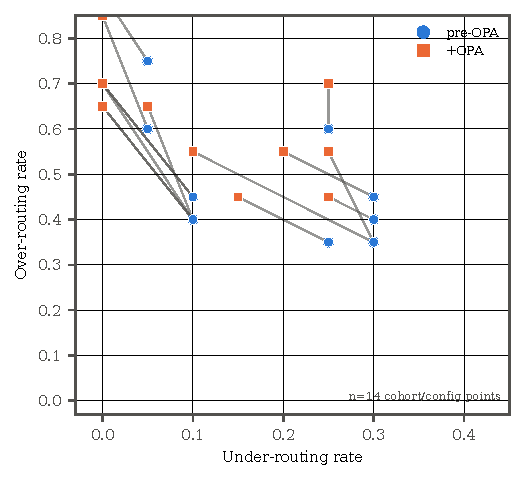
\includegraphics[width=\columnwidth]{figures/fig_routing_tradeoff.pdf}
\caption{Under-routing vs.\ over-routing, before (blue circle) and after (orange square) OPA, for the MAUDE-ECG default model (qwen2.5:3b, development and held-out) and the six representative configurations (development and held-out each), 14 points total. Connecting lines show the per-cohort pre-to-post-OPA movement. Over-routing rises after OPA in all 14 points; under-routing falls in 13 of 14, with one tie (gemma3:1b, development split), visualizing the conservative-routing trade-off reported in Table~\ref{tab:maude-governance} and the six-configuration text above across the full tested set at once.}
\label{fig:routing-tradeoff}
\end{figure}
\fi

\subsubsection{Model-Scale Sensitivity of Symbolic Checks}
\label{sec:model-scale-sensitivity}

We tested whether the Qwen2.5 pattern persists across nine qwen3.5 (0.8B--27B) and gemma3 (1B--27B) configurations under the matched-strict protocol; eight met the prespecified completion criterion.\ifscalingtable{} Table~\ref{tab:scaling-sweep} reports exact values.\fi\ifscalingplot{} Figure~\ref{fig:scaling-sweep-multipanel} compares them.\fi
\ifscalingtable

\begin{table}[t]
\centering
\caption{Two-series scaling sweep: eight completed configurations ($n=40$ each)}
\label{tab:scaling-sweep}
\scriptsize
\setlength{\tabcolsep}{2.0pt}
\begin{tabular}{lp{0.13\columnwidth}p{0.16\columnwidth}p{0.13\columnwidth}p{0.15\columnwidth}}
\hline
\textbf{Model} & \textbf{Severity exact} & \textbf{Union yield} & \textbf{Shared} & \textbf{Genuine SHACL rate} \\
\hline
gemma3:1b & 0.325 & 0.800 & 0.844 & 0.000 \\
qwen3.5:2b & 0.325 & 0.725 & 0.517 & 0.300 \\
gemma3:4b & 0.475 & 0.700 & 0.107 & 0.350 \\
qwen3.5:4b & 0.500 & \textbf{1.000} & \textbf{0.925} & 0.075 \\
gemma3:12b & 0.500 & 0.850 & 0.265 & 0.350 \\
qwen3.5:9b & 0.575 & 0.800 & 0.625 & 0.125 \\
gemma3:27b & 0.750 & \textbf{1.000} & \textbf{0.875} & 0.075 \\
qwen3.5:27b & 0.650 & \textbf{0.125} & 0.000 & 0.000 \\
\hline
\multicolumn{5}{p{0.94\columnwidth}}{\scriptsize qwen3.5:0.8b is excluded because persistent schema-validation failures prevented completion under the prespecified generation protocol. Shared is the fraction of union findings attributable to structurally shared activation; genuine SHACL rate is measured over all 40 scenarios. qwen3.5:2b's values reflect the original run; a same-digest reproduction attempt 72 hours later showed reliability degradation for this configuration (Threats to Validity).} \\
\end{tabular}
\end{table}  \fi

\ifscalingplot

\begin{figure}[t]
\centering
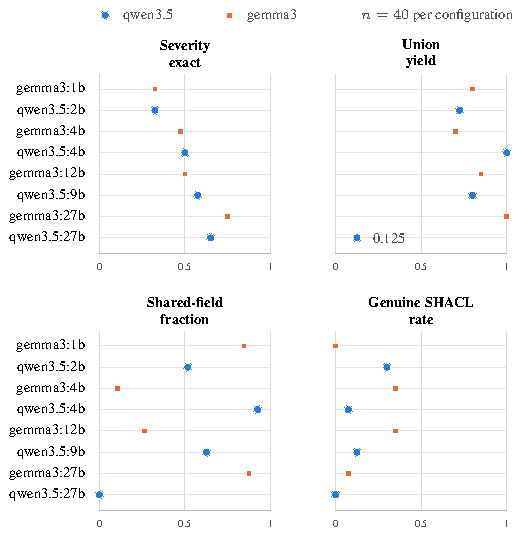
\includegraphics[width=\columnwidth]{figures/fig3_scaling_sweep.pdf}
\caption{Two-series scaling sweep across eight qwen3.5/gemma3 configurations ($n=40$ each): severity-exact accuracy, OPA-or-SHACL union yield, structurally shared-field fraction, and genuine incremental SHACL rate, one dot per model per panel. Color/marker identifies model family (qwen3.5 circle, gemma3 square). qwen3.5:0.8b is excluded after schema-validation failures. qwen3.5:2b values are from the original run; Threats to Validity reports its same-digest re-probe 72 hours later.}
\label{fig:scaling-sweep-multipanel}
\end{figure}  \fi

Union yield is nonmonotonic: it reaches 1.000 at qwen3.5:4b and gemma3:27b, with 87.5--92.5\% structurally shared findings, but falls to 0.125 at qwen3.5:27b. That model still achieves 0.650 severity accuracy (1.000 within one level) without citation hallucinations or retries. Thirteen of its 14 errors are over-calls outside the one-sided \texttt{concept\_severity\_undercall} rule; the sole under-call fires it, and no case has empty \texttt{evidence\_links}. Provenance therefore identifies both detected defects and coverage gaps.

\subsubsection{Cross-Domain Stress Test}
\label{sec:cgm-generalization}

A CGM/insulin-dosing stress test reuses the DAG and report contract with a new policy and curated layer ($n=20$; qwen2.5:3b; three unseeded repeats). No scenario was unsafely under-escalated (95\% Wilson [0.0000,0.1611]); human review was 20/20, severity accuracy 10/20, and recommendation agreement changed from 12/20 before OPA to 10/20 after OPA. Mean Artifact Recall@4 was 0.65, row-macro citation validity 0.9736, and scenario-level validity 19/20. Across 18 runs, severity accuracy ranged from 0.15 to 0.85, Artifact Recall@4 from 0.55 to 0.65, and macro citation validity from 0.91 to 1.00. Assertion-status handling remained the main transfer weakness, while deterministic enforcement separated boundary consistency from model accuracy.

\subsubsection{Paraphrase Robustness}
\label{sec:paraphrase-robustness}

Eight paraphrases of five curated scenarios provide a correlated 40-row stability check. With qwen2.5:3b, governed recommendation agreement was 24/40, OPA-or-SHACL union yield was 19/40 (3 OPA-only, 6 SHACL-only, 10 overlap), all runtime checks passed, and no report crossed the authority boundary. qwen3.5:4b and gemma3:27b reproduced the shared-field pattern (37/37 and 34/34 overlap cases), whereas qwen3.5:27b showed no structural overlap; qwen3.5:0.8B and 2B did not complete because of repeated schema-validation failures.

\section{Case Study and Discussion}
\label{sec:case-study}

A post-market arrhythmia drift alert becomes a typed signal linked to the affected model. The agent retrieves artifacts and records gaps in a cited \textit{RiskReport}; OPA routes it, SHACL checks curated facts, and field provenance identifies complementary findings (Section~\ref{sec:guard-independence}). The stable contract permits generator changes without redefining governance, while production can protect the external gate through policy-as-code controls~\cite{github_environments,opa_cicd}.

\subsection*{Human Decision Rights}

Human-centered operation requires reviewer control of release and access to sources, gaps, confidence, and policy actions. Reviewers can disagree, request evidence, or return a high-risk recommendation that omits required subgroup evidence without treating advice as authorization. Linking each decision to its audit trace also supports future studies of calibrated reliance~\cite{goddard_automation_bias,gaube_do_as_ai_say,tschandl_collaboration}.

\subsection*{Threats to Validity}

\textbf{Internal validity}: scenario similarity creates dependence. Token-Jaccard analysis connected 36 scenarios into 19 clusters; a 1.7--2.0 design effect reduced the effective sample to roughly 20--23 and widened the pooled severity-accuracy interval from [0.285, 0.578] to [0.238, 0.636]. The frozen split and unpinned-seed repeats measure post-freeze behavior and output variance, not additional independent scenarios.

\textbf{External validity}: eight of nine scaling configurations completed; MAUDE, CGM, and paraphrase analyses use subsets, and qwen3.5:0.8B/2B failed the longer paraphrase protocol. The study targets local 1B--27B open-weight models and curated or protocol-derived data, not proprietary models or multi-site deployments; the 0/20 CGM unsafe count retains a 16.11\% upper bound.

\textbf{Construct validity}: developer-authored labels test execution of a loaded governance specification, not clinical authority. MAUDE evaluates OPA but not full SHACL; shared-team annotation and repaired-case reuse may favor the rules. The analyses establish selected architectural properties, not reliance or clinical correctness. Alloy restricts Time to one total order, matching Python BFS and TLA+/TLC; the earlier multi-chain encoding was UNSAT only at partial extended scope. The reformulation aligns the three methods rather than weakening the property, and guarantees remain limited to single-execution-history semantics. Resource profiling beyond generation latency, live integration, authenticated authorization, and production SHACL remain untested. Section~\ref{sec:synthetic-40}'s decomposition isolates which check catches a defect on one report, not agent-vs-fixed-workflow or independently re-executed OPA/SHACL; both remain future work.

\textbf{Model reproducibility}: a same-digest re-probe 72 hours after the original run varied by configuration. qwen3.5:2b (original union yield 0.725) exhausted retries on one split and increased failures on the other (4/40 versus 1/40), a reliability regression without evident outcome changes among completed cases. qwen3.5:9b changed 1/40 governed outcomes and its genuine SHACL rate from 0.125 to 0.200; gemma3:27b retained union yield 1.000 with 0/40 disagreements. Because revision re-invokes the model, claims are bounded to same-digest, same-day conditions. The CGM severity spread (0.20, 0.55, 0.50) likewise exposes sampling variance.

% TODO BLOCCANTE prima della submission: sostituire [ZENODO DOI] con un DOI
% reale e verificare che il deposito sia pubblico (o con link di accesso per i
% reviewer): per un paper la cui tesi e' la riproducibilita', un placeholder
% qui e' un motivo concreto di penalizzazione in review.
\paragraph{Data and code availability.} The package at [ZENODO DOI] contains benchmarks, annotations, models, policies, traces, and scripts that regenerate results from hashed raw outputs under the qualification above. MAUDE annotation files reproduce full source-narrative text from the public FDA MAUDE database (public domain) rather than identifiers alone, so that inter-rater agreement is independently auditable against the underlying narratives.

 \section{Conclusion}

The architecture assigns recommendation and authorization to different objects, actors, and controls. Its \textit{RiskReport} connects a bounded agent to OPA, SHACL, and a modeled external human gate. Within the checked bounds, formal analysis found no counterexample under single-execution-history semantics. Of 2,000 attempted runs, 1,947 terminated under control (1,189 packages; 758 escalations), with no state-illegal action accepted. The evaluations exposed complementary detection and the workload cost of conservative routing---a trade-off that lives in declarative policy and can be recalibrated without touching the agent, contract, or authority boundary. The interface keeps evidence assembly inspectable and distinct from release authority; external indipendent annotation, human evaluation, and authenticated integration remain future work.

% TODO before final submission: add Author Contributions (e.g., CRediT roles) after author responsibilities are finalized.
% TODO before final submission: add an explicit Funding statement, including a no-external-funding statement if applicable

\section*{Acknowledgment}

The authors used OpenAI Codex for language editing, LaTeX formatting, and plotting code. They reviewed and validated all outputs and take full responsibility for the manuscript.

\section*{Conflict of Interest}

The authors declare no conflicts of interest.

\begin{thebibliography}{99}
\sloppy

\bibitem{future_ai}
K. Lekadir et al.,
``FUTURE-AI: International consensus guideline for trustworthy and deployable artificial intelligence in healthcare,''
\textit{BMJ}, vol. 388, Art. no. e081554, Feb. 2025, doi: 10.1136/bmj-2024-081554.

\bibitem{nist_ai_rmf}
E. Tabassi,
\textit{Artificial Intelligence Risk Management Framework (AI RMF 1.0)}, NIST AI 100-1,
National Institute of Standards and Technology, Gaithersburg, MD, USA, Jan. 2023,
doi: 10.6028/NIST.AI.100-1.

\bibitem{eu_ai_act}
European Parliament and Council,
``Regulation (EU) 2024/1689 laying down harmonised rules on artificial intelligence,''
\textit{Official Journal of the European Union}, L 2024/1689, Jul. 12, 2024.
[Online]. Available: \url{https://eur-lex.europa.eu/eli/reg/2024/1689/oj/eng}

\bibitem{fda_aiml_2021}
U.S. Food and Drug Administration,
``Artificial intelligence/machine learning (AI/ML)-based software as a medical device (SaMD) action plan,'' Jan. 2021.
[Online]. Available: \url{https://www.fda.gov/medical-devices/software-medical-device-samd/artificial-intelligencemachine-learning-aiml-based-software-medical-device-samd-action-plan}.

\bibitem{fda_pccp_2025}
U.S. Food and Drug Administration,
``Marketing submission recommendations for a predetermined change control plan for artificial intelligence-enabled device software functions,''
Final Guidance for Industry and FDA Staff, Dec. 2024.
[Online]. Available: \url{https://www.fda.gov/regulatory-information/search-fda-guidance-documents/marketing-submission-recommendations-predetermined-change-control-plan-artificial-intelligence}.

\bibitem{eu_mdr}
European Parliament and Council,
``Regulation (EU) 2017/745 on medical devices,''
\textit{Official Journal of the European Union}, L 117, pp. 1--175, May 5, 2017.

\bibitem{future_ai_review}
G. Kondylakis et al.,
``A review of methods for trustworthy AI in medical imaging: The FUTURE-AI guidelines,''
\textit{IEEE J. Biomed. Health Inform.}, vol. 30, no. 3, pp. 2299--2315, Mar. 2026,
doi: 10.1109/JBHI.2025.3614546.

\bibitem{iso13485}
\textit{Medical Devices---Quality Management Systems---Requirements for Regulatory Purposes},
ISO 13485:2016, International Organization for Standardization, Geneva, Switzerland, 2016.

\bibitem{iso14971}
\textit{Medical Devices---Application of Risk Management to Medical Devices},
ISO 14971:2019, International Organization for Standardization, Geneva, Switzerland, 2019.

\bibitem{iso42001}
\textit{Information Technology---Artificial Intelligence---Management System},
ISO/IEC 42001:2023, International Organization for Standardization/International Electrotechnical Commission, Geneva, Switzerland, 2023.

\bibitem{fda_gmlp}
U.S. Food and Drug Administration, Health Canada, and U.K. Medicines and Healthcare products Regulatory Agency,
``Good machine learning practice for medical device development: Guiding principles,'' Oct. 2021.
[Online]. Available: \url{https://www.fda.gov/media/153486/download}.

\bibitem{nist_genai_profile}
National Institute of Standards and Technology,
\textit{Artificial Intelligence Risk Management Framework: Generative Artificial Intelligence Profile}, NIST AI 600-1,
Gaithersburg, MD, USA, Jul. 2024, doi: 10.6028/NIST.AI.600-1.

\bibitem{decide_ai}
B. Vasey et al.,
``Reporting guideline for the early-stage clinical evaluation of decision support systems driven by artificial intelligence: DECIDE-AI,''
\textit{Nature Med.}, vol. 28, no. 5, pp. 924--933, May 2022, doi: 10.1038/s41591-022-01772-9.

\bibitem{economou_zavlanos_jamia}
N. J. Economou-Zavlanos et al.,
``Translating ethical and quality principles for the effective, safe and fair development, deployment and use of artificial intelligence technologies in healthcare,''
\textit{J. Amer. Med. Inform. Assoc.}, vol. 31, no. 3, pp. 705--713, Mar. 2024, doi: 10.1093/jamia/ocad221.

\bibitem{wang_governance_scoping}
A. Wang, S. Freeman, and F. Magrabi,
``Governance for safe and responsible AI in healthcare organisations: A scoping review of frameworks,''
\textit{npj Digit. Med.}, vol. 9, Art. no. 516, May 2026, doi: 10.1038/s41746-026-02679-2.

\bibitem{toivakka_regops}
H. Toivakka, T. Granlund, T. Poranen, and Z. Zhang,
``Towards RegOps: A DevOps pipeline for medical device software,''
in \textit{Product-Focused Software Process Improvement}, LNCS 13126,
Cham, Switzerland: Springer, 2021, pp. 290--306,
doi: 10.1007/978-3-030-91452-3\_20.

\bibitem{mirto_biodevops_phdforum}
F. O. Mirto,
``PhD Forum: BioDevOps: Toward a formal framework for continuous deployment in safety-critical medical devices,''
in \textit{Proc. 2026 IEEE Int. Conf. Smart Computing Workshops and Other Affiliated Events (SmartComp Companion)},
2026, pp. 424--426,
doi: 10.1109/SmartComp-Companion70724.2026.00094.

\bibitem{lewis_rag}
P. Lewis et al.,
``Retrieval-augmented generation for knowledge-intensive NLP tasks,''
in \textit{Advances in Neural Information Processing Systems 33}, 2020,
pp. 9459--9474.

\bibitem{yao_react}
S. Yao et al.,
``ReAct: Synergizing reasoning and acting in language models,''
in \textit{Proc. 11th Int. Conf. Learn. Representations}, Kigali, Rwanda, May 2023.

\bibitem{agentic_taxonomy_2026}
S. Vatsal, H. Dubey, and A. Singh,
``Agentic AI in healthcare and medicine: A seven-dimensional taxonomy for empirical evaluation of LLM-based agents,''
arXiv preprint arXiv:2602.04813, Feb. 2026.

\bibitem{agentclinic}
S. Schmidgall et al.,
``AgentClinic: A multimodal agent benchmark to evaluate AI in simulated clinical environments,''
arXiv preprint arXiv:2405.07960, May 2024.

\bibitem{medagentbench}
Y. Jiang et al.,
``MedAgentBench: A realistic virtual EHR environment to benchmark medical LLM agents,''
arXiv preprint arXiv:2501.14654, Jan. 2025.

\bibitem{agentic_limits_2026}
G. Ar\'anguiz Dias et al.,
``The doctor will (still) see you now: On the structural limits of agentic AI in healthcare,''
arXiv preprint arXiv:2602.18460, Feb. 2026.  \bibitem{garmle_g}
W. Li et al.,
``Refine medical diagnosis using generation augmented retrieval and clinical practice guidelines,''
\textit{IEEE J. Biomed. Health Inform.}, early access, Dec. 2025,
doi: 10.1109/JBHI.2025.3641931.

\bibitem{public_ehr_benchmark}
K. Yu et al.,
``Benchmarking foundation models with multimodal public electronic health records,''
\textit{IEEE J. Biomed. Health Inform.}, early access, Dec. 2025,
doi: 10.1109/JBHI.2025.3645076.



\bibitem{goddard_automation_bias}
K. Goddard, A. Roudsari, and J. C. Wyatt,
``Automation bias: A systematic review of frequency, effect mediators, and mitigators,''
\textit{J. Amer. Med. Inform. Assoc.}, vol. 19, no. 1, pp. 121--127, Jan. 2012,
doi: 10.1136/amiajnl-2011-000089.

\bibitem{gaube_do_as_ai_say}
S. Gaube et al.,
``Do as AI say: Susceptibility in deployment of clinical decision-aids,''
\textit{npj Digit. Med.}, vol. 4, Art. no. 31, Feb. 2021,
doi: 10.1038/s41746-021-00385-9.

\bibitem{tschandl_collaboration}
P. Tschandl et al.,
``Human--computer collaboration for skin cancer recognition,''
\textit{Nature Med.}, vol. 26, no. 8, pp. 1229--1234, Aug. 2020,
doi: 10.1038/s41591-020-0942-0.

\bibitem{liu_snomed_kg}
D. Liu et al.,
``SNOMED CT-powered knowledge graphs for structured clinical data and diagnostic reasoning,''
arXiv preprint arXiv:2510.16899, Oct. 2025.

\bibitem{fhir}
HL7 International,
``FHIR Release 4: Fast Healthcare Interoperability Resources.''
[Online]. Available: \url{https://hl7.org/fhir/R4/}.

\bibitem{snomed}
SNOMED International,
``SNOMED CT Starter Guide.''
[Online]. Available: \url{https://confluence.ihtsdotools.org/display/DOCSTART}.

\bibitem{shacl}
World Wide Web Consortium,
``Shapes Constraint Language (SHACL),'' W3C Recommendation, Jul. 20, 2017.
[Online]. Available: \url{https://www.w3.org/TR/shacl/}.

\bibitem{owl2}
World Wide Web Consortium,
``OWL 2 Web Ontology Language document overview,'' W3C Recommendation, Dec. 11, 2012.
[Online]. Available: \url{https://www.w3.org/TR/owl2-overview/}.  \bibitem{leucker_runtime}
M. Leucker and C. Schallhart,
``A brief account of runtime verification,''
\textit{J. Log. Algebr. Program.}, vol. 78, no. 5, pp. 293--303, May--Jun. 2009,
doi: 10.1016/j.jlap.2008.08.004.

\bibitem{opa_cicd}
Open Policy Agent,
``Policy-based control for cloud native environments.''
[Online]. Available: \url{https://www.openpolicyagent.org/}.

\bibitem{github_environments}
GitHub Docs,
``Managing environments for deployment.''
[Online]. Available: \url{https://docs.github.com/actions/deployment/targeting-different-environments/managing-environments-for-deployment}.



\bibitem{nemo_guardrails}
T. Rebedea, R. Dinu, M. N. Sreedhar, C. Parisien, and J. Cohen,
``NeMo Guardrails: A toolkit for controllable and safe LLM applications with programmable rails,''
in \textit{Proc. 2023 Conf. Empirical Methods Natural Language Processing: System Demonstrations},
Singapore, Dec. 2023, pp. 431--445, doi: 10.18653/v1/2023.emnlp-demo.40.

\bibitem{agentspec}
H. Wang, C. M. Poskitt, and J. Sun,
``AgentSpec: Customizable runtime enforcement for safe and reliable LLM agents,''
in \textit{Proc. 48th IEEE/ACM Int. Conf. Softw. Eng. (ICSE)},
Rio de Janeiro, Brazil, Apr. 12--18, 2026, 12 pp.,
doi: 10.1145/3744916.3764546.

\bibitem{iec62304}
\textit{Medical Device Software---Software Life Cycle Processes},
IEC 62304:2006+AMD1:2015, International Electrotechnical Commission,
Geneva, Switzerland, 2015.

\bibitem{fda_maude}
U.S. Food and Drug Administration,
``Manufacturer and User Facility Device Experience (MAUDE) Database.''
[Online]. Available: \url{https://www.accessdata.fda.gov/scripts/cdrh/cfdocs/cfmaude/search.cfm}.

\fussy
\end{thebibliography}

\end{document}